\documentclass{article}
\usepackage{amsmath}
\usepackage[utf8]{inputenc}
\usepackage{float}
\usepackage{epsfig,graphicx}
\usepackage{xcolor,import}
\usepackage[german]{babel}
\usepackage{textcomp}
\usepackage{mathtools}

\begin{document}
\thispagestyle{empty}
			\begin{center}
			\Large{Fakultät für Physik}\\
			\end{center}
\begin{verbatim}


\end{verbatim}
							%Eintrag des Wintersemesters
			\begin{center}
			\textbf{\LARGE WINTERSEMESTER 2014/15}
			\end{center}
\begin{verbatim}


\end{verbatim}
			\begin{center}
			\textbf{\LARGE{Physikalisches Praktikum 1}}
			\end{center}
\begin{verbatim}




\end{verbatim}

			\begin{center}
			\textbf{\LARGE{PROTOKOLL}}
			\end{center}
			
\begin{verbatim}





\end{verbatim}

			\begin{flushleft}
			\Large{\textbf{Experiment Nr. 6:} Geometrische Optik}\\
							%Experiment Nr. und Titel statt den Punkten eintragen
			\LARGE{}	
			\end{flushleft}

\begin{verbatim}

\end{verbatim}	
							%Eintragen des Abgabedatums, oder des Erstelldatums des Protokolls
			\begin{flushleft}
			\textbf{\Large{Datum:}} \Large{21.11.2014}
			\end{flushleft}
			
\begin{verbatim}
\end{verbatim}
							%Namen der Protokollschreiber
		\begin{flushleft}
			\textbf{\Large{Namen:}} \Large{Veronika Bachleitner, Erik Grafendorfer}
			\end{flushleft}

\begin{verbatim}


\end{verbatim}
							%Kurstag und Gruppennummer, zb. Fr/5
			\begin{flushleft}
			\textbf{\Large{Kurstag/Gruppe:}} \Large{Fr/1}
			\end{flushleft}

\begin{verbatim}






\end{verbatim}
							%Name des Betreuers, das Praktikum betreute.
			\begin{flushleft}
			\LARGE{\textbf{Betreuer:}}	\Large{Stana}	
			\end{flushleft}
\newpage	

\section{Brennweite von Linsen}

\subsection{Aufgabenstellung}
Wir bestimmen die Brennweiten und die Brechkraft von einer Konvexlinse und einer Konkavlinse.
\subsection{Grundlagen}
Wir verwenden die \textbf{Abbildungsgleichung für Linsen:}
\begin{equation}
\label{linsengleichung}
\frac{1}{f}=\frac{1}{g}+\frac{1}{b}
\end{equation}
$\frac{1}{f}$ ist die Brechkraft der Linse und wird in Dioptrien ([1/m]) angegeben. f ist die Brennweite, g die Gegenstandsweite, b die Bildweite.\\ 
\\
Wir verwenden auch das \textbf{Besselverfahren}, das sich durch eine Distanz zwischen Schirm und Gegenstand von einem Minimum vom vierfachen der Brennweite der zu untersuchenden Linse charakterisiert. Durch es ergibt sich die Brennweite f zu 
\begin{equation}
\label{bessel}
f=\frac{1}{4}(e-\frac{d^2}{e})
\end{equation}
wobei e die Distanz zwischen Schirm und Gegenstand und d die Distanz zwischen den beiden Positionen der Linse bezeichnet, an denen sie ein scharfes Bild liefert.
\subsection{Versuchsaufbau und Methoden}
Wir haben eine Schiene mit verschiebbaren Linsen. Darauf ist eine Lichtquelle, vor der wir einen Gegenstand platzieren. Dieser wird durch die Linsen auf einen verschiebbaren Schirm abgebildet. Wir verschieben den Schirm und die Linsen auf Positionen auf denen sich scharfe Bilder ergeben und messen ihre Distanzen; aus diesen ermitteln wir die Eigenschaften der Linsen.
\subsection{Durchführung}
Bei der Durchführung gelang es uns trotz Hilfe nicht, ein scharfes Bild mit der Konkavlinse zu erzeugen. Wir müssen diesen Punkt daher streichen	, da sich keine Ergebnisse präsentierten, die im Reich der Vernunft anzusiedeln wären.
\subsection{Ergebnisse}
\subsubsection*{Brennweite und Brechkraft einer Konvexlinse}
\paragraph{Bei einer Gegenstandsweite}

Wir messen 5 Mal die Bildweite b bei fixer Gegenstandsweite und berechnen den Mittelwert sowie seine Standardabweichung.

$$\bar{b}=(0.65 \pm 0.005)m$$

Da seine Unsicherheit, die Standardabweichung, 5 mal größer ist als die Unsicherheit der Gegenstandsweite von $\pm 0.001m$, verwenden wir nur diese bei der Berechnung der Unsicherheit der Brechkraft mit dem Gaußschen Fehlerfortpflanzungsgesetz. \\
Mittels (\ref{linsengleichung}) erhalten wir:\\
\boxed{$$f=(0.0971 \pm 0.007) m$$}\\
\boxed{$$\frac{1}{f}=(10.30 \pm 0.7) Dioptrien$$}
\paragraph{Besselverfahren}
Wir messen 5 Paare von Distanzen zwischen den beiden scharfen Positionen der Linse, d, und zwischen Schirm und Gegenstand, e. Daraus berechnen wir mittels (\ref{bessel}) die 5 zugehörigen Brennweiten und ermitteln ihren Mittelwert.\\
\boxed{$$\bar{f}=(0.0963\pm 0.002)m$$}\\
\boxed{$$\frac{1}{\bar{f}}=(10.4 \pm 0.3) Dioptrien $$}
\begin{center}
\begin{figure}
\caption{Strahlengang bei der Konkavlinse}
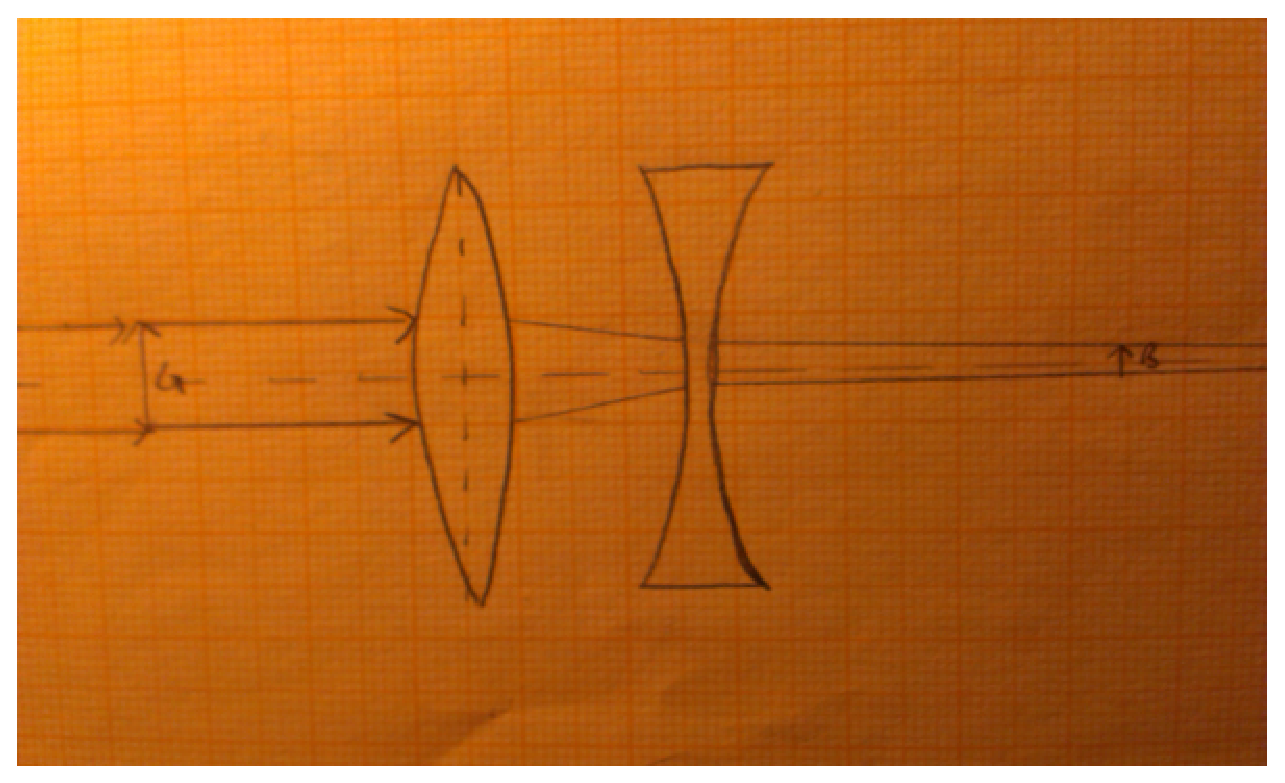
\includegraphics[scale=0.5]{graph3.eps}
\end{figure}
\end{center}
\subsection{Diskussion}
Das Besselverfahren liefert ein genaueres Ergebnis. Es liegt aber im Vertrauensbereich unseres anderen Ergebnisses - also können wir vertrauen dass wir mit beiden Methoden gut gemessen haben!\\
Für die Konkavlinse können wir wie schon erwähnt leider kein glaubwürdiges Ergebnis angeben - unser einziger Messwert legt uns eine Brennweite von -2mm nahe, was uns als sehr falsch erklärt wurde. 
\section{Linsenfehler}

\subsection{Aufgabenstellung}
Wir bestimmen die sphärische Aberration einer dicken Linse in den Durchgangsrichtungen plan-konvex und konvex-plan.
\subsection{Grundlagen}
Dadurch, dass achsennahe und achsenferne Strahlen in unterschiedlichen Winkeln auf die Linsenzonen fallen, werden sie in unterschiedlichen Brennpunkten gebrochen. Diesen Fehler nennt man sphärische Aberration.
\subsection{Versuchsaufbau und Methoden}
Wir haben eine dicke, plankonvexe Linse auf die wir durch verschiedene Schlitzblenden Licht fallen lassen. Dieses Licht wurde zuvor mit einer Hilfslinse in annähernd parallele Lichtbündel gebrochen. Durch die unterschiedliche Entfernung von der Achse der einzelnen Schlitze werden die durchgelassenen Strahlen in unterschiedlichen Brennpunkten zusammengeführt. Wir beobachten dies auf einem verschiebbaren Schirm - und messen die Position des Schirms, bei der die Strahlen aus einer Schlitzkonfiguration scharf zusammenfallen. \\
Wir drehen nach dem ersten Durchgang die Linse aus plankonvexer Durchgangsrichtung zu konvexplaner um.
\subsection{Durchführung}
Bei der Durchführung ergaben sich keine Schwierigkeiten.
\subsection{Ergebnisse}
plan-konvex:\\
Die Hauptebene der Linse befindet sich im Punkt: $(0.615 \pm 0.005)mm$\\
3 Brennpunkte:\\
Enge Schlitze: $(0.748 \pm 0.001)mm$\\
Mittlere Schlitze: $(0.736 \pm 0.001)mm$\\
Weite Schlitze: $(0.705 \pm 0.001)$\\
\\
konvex-plan:\\
Die Hauptebene der Linse befindet sich im Punkt: $(0.615 \pm 0.002)mm$\\
3 Brennpunkte:
Enge Schlitze: $(0.695 \pm 0.001)mm$\\
Mittlere Schlitze: $(0.689 \pm 0.001)mm$\\
Weite Schlitze: $(0.683 \pm 0.001)$\\
\begin{center}
\begin{figure}
\caption{Plan-Konvexe Richtung}
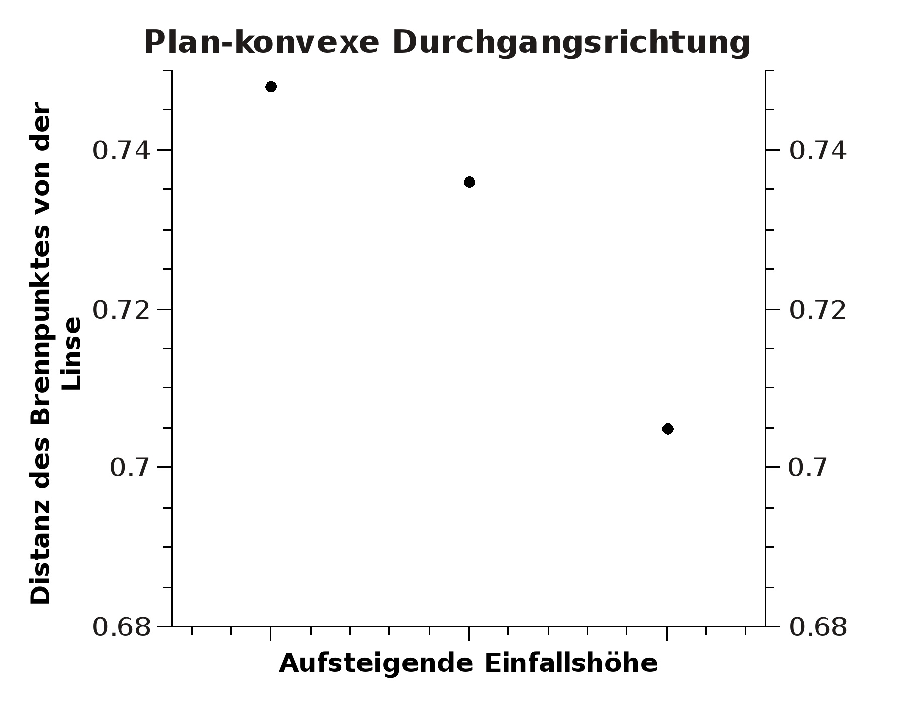
\includegraphics[scale=0.7]{graph1.eps}
\end{figure}
\end{center}
\begin{center}
\begin{figure}
\caption{Konvex-Plane Richtung}
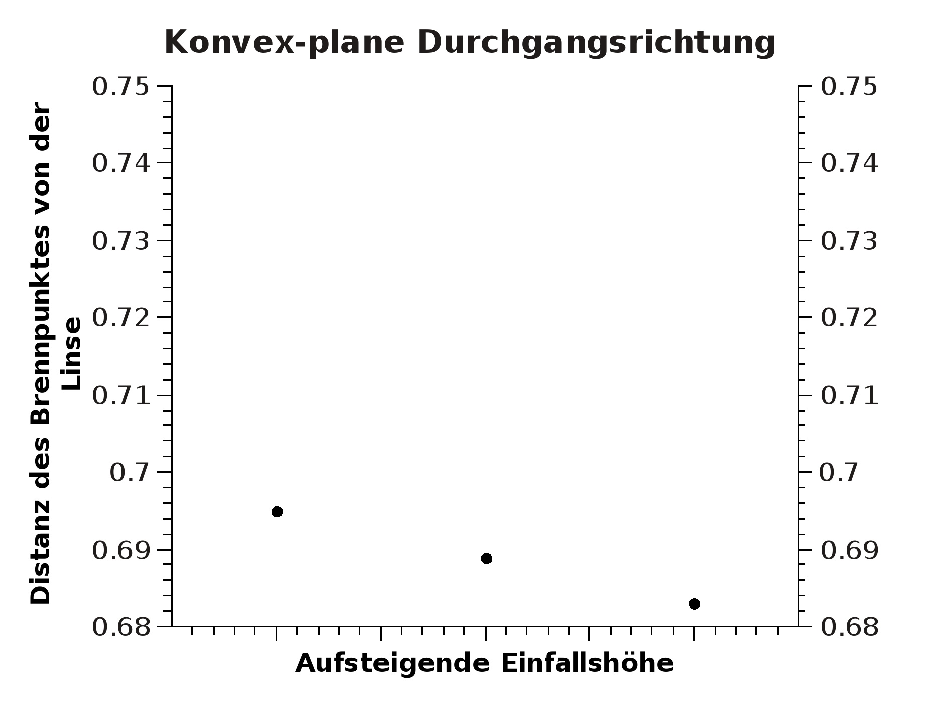
\includegraphics[scale=0.7]{graph2.eps}
\end{figure}
\end{center}
\subsection{Diskussion}
Aus den Messungen zeigt sich, dass die Durchgangsrichtung konvex-plan weniger Fehler aufweist. Dies liegt daran, dass das Licht in diesem Fall zweimal gebrochen wird: Einmal durch die konvexe, einmal durch die plane Ebene. \\
In die andere Richtung ist das nicht so, da das Licht im Anfang durch die plane Ebene geht und hier nicht gebrochen wird. Dadurch stellt sich ein größerer Fehler aufgrund der konvexen Ebene ein. \\
In unseren beiden Abbildungen haben wir die Ordinaten im selben Bereich von 0.68 m bis 0.75 m geplotted, damit man sofort sehen kann, dass bei konvex-planer Durchgangsrichtung die Brennpunkte näher an der Linse und näher aneinander liegen als bei plan-konvexer Richtung - wie erwartet. Dabei zeigt vor allem die geringere Distanz zwischen den Punkten selbst dass der Fehler geringer ist, da das bedeutet dass die Brennpunkte näher aneinander liegen. 



\section{Mikroskop}

\subsection{Aufgabenstellung}
Wir bauen ein Mikroskop mithilfe zweier Konvexlinsen kleiner Brennweiten. Wir messen die Gesamtvergrößerung mithilfe einer Strichplatte als Gegenstand und testen die Abhängigkeit der Vergrößerung von der Tubuslänge. \\
Außerdem messen wir die Dicke eines Haares mit unserem Aufbau.
\subsection{Grundlagen}
Berechnung der Tubuslänge aus den Brennweiten und des Abstands der Linsen: $t=d-f_{Ob}-f_{Ok}$\\
Berechnung der Vergrößerung: $V_M=\frac{t_1}{f_{Ob}}\frac{s_0}{f_{Ok}}$
\subsection{Versuchsaufbau und Methoden}
Wir haben einen Bausatz mit verschiedenen Linsen. Wir wählen zwei aus und befestigen sie an dünnen Stangen in einem fixen Abstand zueinander. Dann bewegen wir die beiden Linsen gemeinsam hin und her, bis wir den Punkt finden, an dem sie ein scharfes Bild ergeben. Von dort messen wir dann ihre Vergrößerung durch Vergleich eines Millimetermaßstabs, gesehen durch das Mikroskop, mit Millimeterpapier, gleichzeitig unvergrößert gesehen mit dem anderen Auge. \\
Dann verändern wir die Distanz der Linsen zueinander und damit die Tubuslänge und wir wiederholen die Messung.
\subsection{Durchführung}
Es war sehr mühsam die beiden verschiedenen Millimetermaße gleichzeitig anzuvisieren und genau abzulesen. 
\subsection{Ergebnisse}
Brennweite der als Objektiv verwendeten Linse: $f_{Ob}=25mm$\\
Brennweite der als Okular verwendeten Linse: $f_{Ok}=40mm$\\
Abstände der Linsen: $d_1=(93 \pm 1)mm$, $d_2=(77 \pm 1)mm$, $d_3=(85 \pm 1)mm$\\
Daraus die Tubuslängen: $t_1=(28 \pm 1)mm$, $t_2=(12 \pm 1)mm$, $t_3=(20 \pm 1)mm$ \\
Berechnete Vergrößerung: 
\begin{gather*}
V_{M_1}=7\\
V_{M_2}=3\\
V_{M_3}=5
\end{gather*}
\\
Gemessene Vergrößerung:\\
Für die erste Tubuslänge entsprechen 20 Einheiten auf der Skala  unter dem Mikroskop, die 10mm/200 Einheiten zählt, 5mm auf dem Papier ohne Mikroskop. Daraus ergibt sich eine Vergrößerung: $$\boxed{V_{M_1}=5 \pm 0.5}$$
Für die zweite Tubuslänge entsprechen 30 Einheiten auf der Skala  5mm. Daraus ergibt sich eine Vergrößerung: $$\boxed{V_{M_2}=3.3 \pm 0.5}$$
Für die dritte Tubuslänge entsprechen 23 Einheiten auf der Skala  5mm. Daraus ergibt sich eine Vergrößerung: $$\boxed{V_{M_3}=4.3 \pm 0.5}$$
\\
Messung der Dicke eines Haares:\\
Das Haar ist 2 Einheiten dick: Dies entspricht bei der Vergrößerung $V_{M_3}$ einer Dicke von: 
$$\boxed{d=(0.1 \pm 0.05)mm}$$
\subsection{Diskussion}
Die Diskrepanzen zwischen den vorhergesagten und den gemessenen Vergrößerungen erklären wir aus der Schwierigkeit die beiden Maßstäbe gleichzeitig zu vergleichen. Aber sie folgen immerhin dem selben Trend: 7/3/5 zu 5/3.3/4.3 oder hoch/niedrig/mittel. 
\section{Fernrohr}
\subsection{Aufgabenstellung}
Wir bauen ein Keplersches und ein Galileisches Fernrohr und bestimmen die erreichte Fernrohrvergrößerung.
\subsection{Grundlagen}
Ein Fernrohr besteht aus einem Objektiv und einem Okular, die in einem bestimmten Abstand voneinander positioniert sind.\\
Ein Keplersches (astronomisches) Fernrohr besteht aus zwei Sammellinsen. Dadurch entsteht ein umgekehrtes Bild. Angenehmer ist das Galileische (holländische) Fernrohr, dass das Bild durch Verwendung einer Sammel- und einer Zerstreuungslinse "richtig herum" darstellt.\\
\\
Die Fernrohrvergrößerung wird mit folgender Formel berechnet: 
$$V_F=\frac{f_{Ob}}{f_{Ok}}$$
\subsection{Ergebnisse}
\textbf{Keplersches Fernrohr:}
Brennweite der als Objektiv verwendeten Linse: $f_{Ob_K}=160mm$\\
Brennweite der als Okular verwendeten Linse: $f_{Ok_K}=120mm$\\
Berechnete Vergrößerung: 1.3\\
Beobachtete Vergrößerung: $1.5 \pm 0.5$\\
\\
\textbf{Galileisches Fernrohr:}
Brennweite der als Objektiv verwendeten Linse: $f_{Ob_G}=160mm$\\
Brennweite der als Okular verwendeten Linse: $f_{Ok_G}=50mm$\\
Berechnete Vergrößerung: 3.2\\
Beobachtete Vergrößerung: $3.0 \pm 0.5$\\

\subsection{Diskussion}
Die Ergebnisse passen sehr gut zu den berechneten Werten.\\
Bei der Beobachtung selbst haben wir aber zuerst das Problem, dass die Experimentatoren verschiedene Vergrößerungen wahrnehmen: Im ersten Fall eine Vergrößerung von 2.5 und eine von 1.5. Dieses Mysterium klärt sich durch die Beobachtung auf, dass ersterer selbst eine sehr starke Brille trägt und so eine weitere Vergrößerung stattfindet, bevor das Bild an seinem Auge angelangt.\\
Wir können dieses Phänomen glücklicherweise weiter testen: Die Experimentatorin trägt an diesem Praktikumstag Kontaktlinsen, hat jedoch ihre Brille dabei. Beim Vergleich zwischen Beobachtung mit Kontaktlinsen bzw. Brille bestätigt sich unsere Theorie.\\
Wir verwenden daher die Beobachtungen, die von der Kontaktlinsen-tragenden Experimentatorin durchgeführt werden können.\\
Wir schreiben eine Unsicherheit von 0.5 Einheiten, da die Experimentatorin keine der Distanz wahrhaft genügenden Kontaktlinsen trägt und daher mit dem Auge, das den Maßstab direkt anvisiert nicht scharf genug sehen kann. Wir wissen nicht, ob andere Gruppen (mitsamt Unsicherheit) präzisere Messergebnisse aufgrund ihrer Sehkraft erreichen können.
\end{document}
